\documentclass[titlepage,hidelinks,10pt]{article}
\usepackage[utf8]{inputenc}
\usepackage{parskip}
\usepackage[UKenglish]{babel}
\usepackage[headheight=15pt,margin=3cm]{geometry}
\usepackage{multicol}
\usepackage{multirow}
\usepackage[colorlinks=false]{hyperref}
\usepackage{float}
\usepackage[toc,page]{appendix}
\usepackage[table]{xcolor}
\usepackage{titling}
\usepackage{array}

\usepackage{color}
\usepackage{listings}
\usepackage{graphicx}
\graphicspath{ {img/} }
\usepackage{caption}
\usepackage{wrapfig}
\usepackage{lscape}
\usepackage{rotating}
\usepackage{epstopdf}
\usepackage{pifont}
\usepackage{gensymb}

\setlength{\parindent}{2em}

\date{January 2017}
\title{Augmented Reality Debugging System for Swarm Robotics \vspace{1cm}\\\Large{Initial Report}}
\author{Alistair Jewers}

\begin{document}

\maketitle

\tableofcontents
\newpage

\section{Project Overview and Aims} \label{Overview}
Swarm Robotics is the name given to the nascent field of study focusing on the use of concepts derived from the study of social insects, such as ants or bees, to design and implement behavioural algorithms for multi-robot systems\cite{InspirationToApplication}. These behaviours should allow a group of relatively simple robots to achieve a more complex, emergent behaviour, through cooperation. The broader area of study, without the robotics focus, is referred to as Swarm Intelligence (SI), and is described by Dorigo \& Birattari as the \textit{``discipline that deals with natural and artificial systems composed of many individuals that coordinate using decentralized control and self-organization''}\cite{SwarmIntelligence}, with examples including insect colonies, fish schools, and flocks of birds. Whilst the details of this complex area of study are outside the scope of this report, it is of importance to the nature of the project to note that one of the key aims of swarm robotics is decentralised control. To this end, in a swarm robotic system you would not expect to find any master controller or central decision making unit. Instead, each robot acts based purely on information available locally, and no point in the system is aware of the current state of all the robots. Also of note is the fact that the state of a robot may change rapidly over time, and be dependent on a large number of environmental or outside factors. Considering these two statements together, it becomes readily apparent that debugging a swarm robotic system may present an enormous challenge, as the state of the system will be complex and rapidly changing, and no single point in the system can provide the user with the complete state information of the system. 

This project, entitled `\textit{Augmented Reality Debugging System for Swarm Robotics}', focuses on the design and implementation of a computer application for monitoring and debugging swarm robotics systems in real time. This will include the use of an existing video based tracking system to monitor the robots' positions. The robots will communicate information regarding their current internal state, sensor readings, and other decision critical data to the computer wirelessly. Graphical representations of the spatial elements of the robots' data will then be overlayed on top of the video feed, whilst non-spatial data will be represented in other forms. By fusing the data from these two sources and presenting it to the user in a combination of graphical and textual formats, the software will aim to allow the user (most likely the researcher running the swarm robotics experiment) to isolate faults in the system more quickly, and determine if the nature of a problem is related to the behaviour under test, or another factor such as sensor/actuator malfunction, incorrect state transition, \textit{etc}. Another aim of the project is to provide this debugging facility in a highly modularised way, which can be incorporated into a swarm robotics system with relative ease. The system will initially target the widely used e-puck\cite{EPuck} robotics platform, but will aim to be designed in a way that allows support for other robots to be incorporated without modifying the core system. Figure \ref{fig:SystemArchitecture} shows a logical representation of the expected system architecture, utilising the e-puck platform.

\begin{figure}[H]
	\begin{center}
	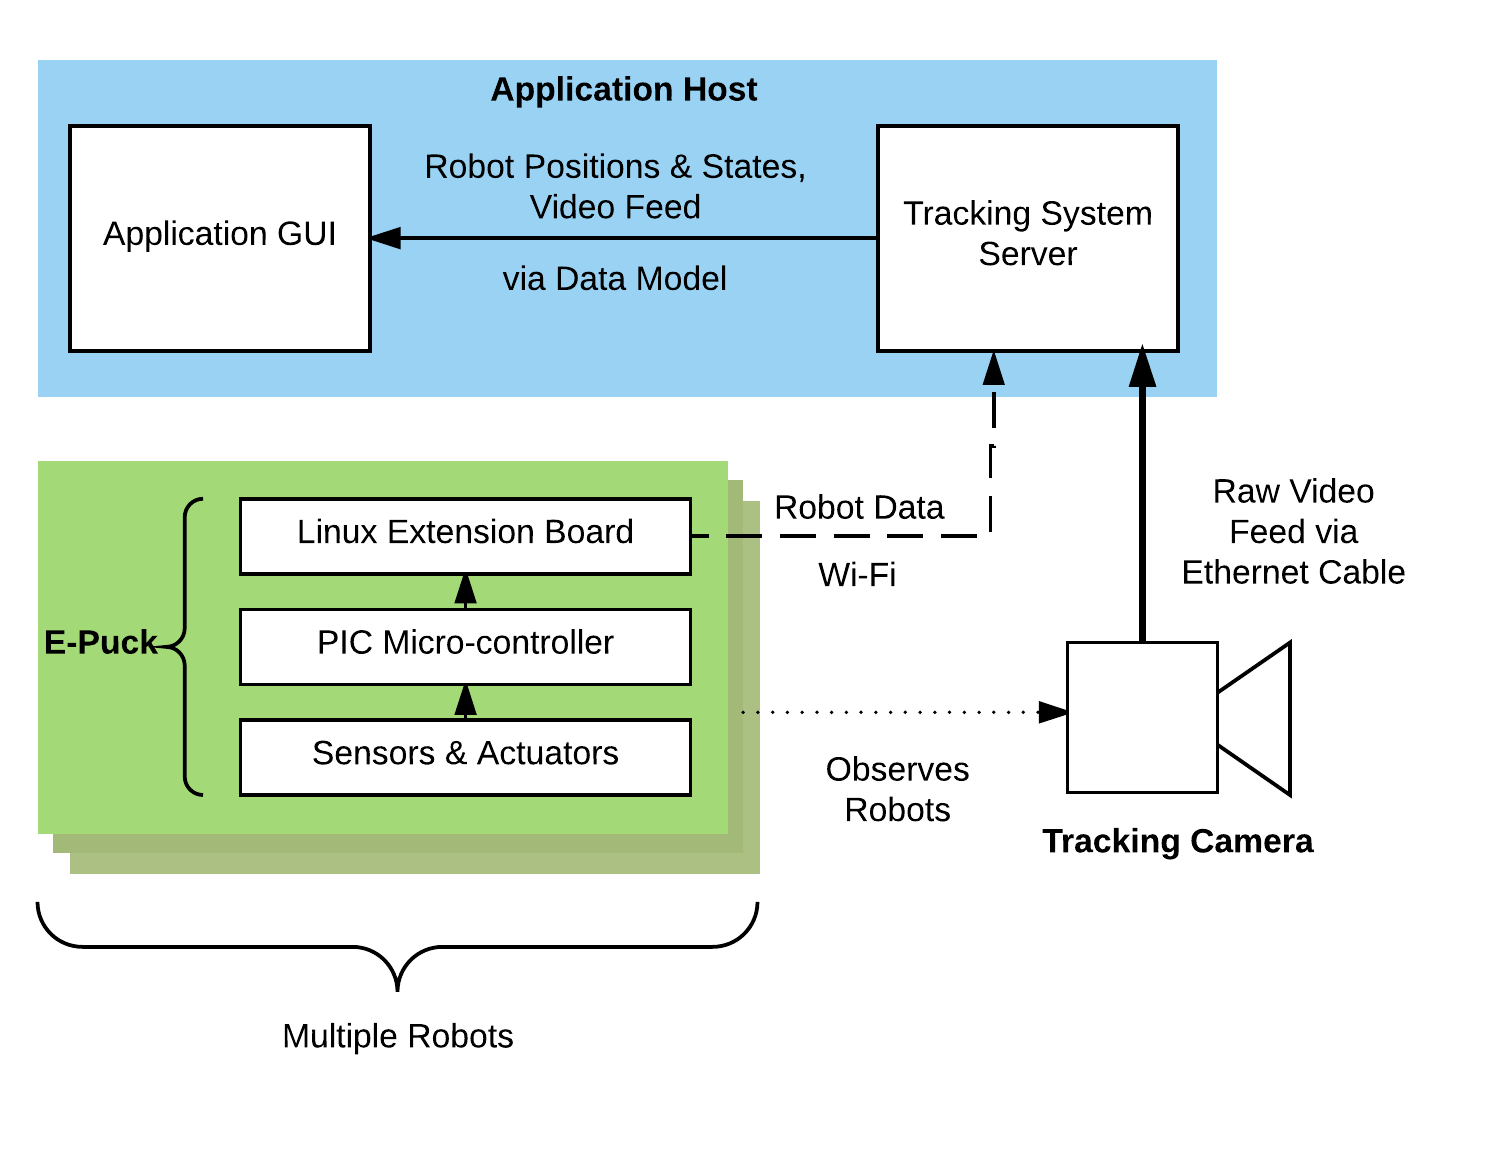
\includegraphics[scale=0.8]{SystemArchitecture.png}
	\caption{Expected general system architecture}
	\label{fig:SystemArchitecture}
	\end{center}
\end{figure}

\section{Literature Survey} \label{LitSurvey}
A number of key areas of literature have been identified as relevant to this project. An understanding of the fundamental concepts of Swarm Robotics, and to a lesser extent Swarm Intelligence, will be key to producing an application that is useful in practice. An overview of the core concepts as well as some key publications are presented in Section \ref{GeneralSR}. A deep understanding of the technical details of specific swarm systems, such as specific behavioural algorithms or implementation details, is not a priority for this project, as the application aims to be more broadly applicable to a wide range of swarm systems. Hence, emphasis is therefore placed on the general classification of swarm robotic systems, relevant problem domains, and recurring concepts, so that the software might better serve researchers in the field.

A relevant area of current research is Human-Swarm Interaction (HSI) - determining how best to interface humans with swarm systems in various roles. This presents two key challenges: the first being how to allow a human operator to provide input and direction to a swarm system without breaking the decentralised control paradigm\cite{HumanSwarmInteractionSurvey}, and the second being how to retrieve data from a swarm system in a coherent form that a human might easily understand\cite{DesginingInterfaces}. This project will be focusing on the latter problem in the context of debugging a swarm system, with the human in a developer role, rather than a user or researcher role where they would be focused on the systems intended output. Despite this perspective difference, HSI research remains highly relevant and must inform the design of the application. An overview of the Human-Swarm Interaction literature is presented in Section \ref{HumanSwarmInteraction}.

Recent advances in virtual-reality (VR) and augmented-reality (AR) technologies have led to an increased interest in using these technologies in conjunction with robotics. AR especially presents a powerful tool for HSI, as an augmented space can be readily understood by both humans and robots. Research relating to the use of AR with robotic systems is summarized in Section \ref{VRAndAR}, alongside a summary of the work currently existing which utilizes these concepts in the context of multi-robot systems, and other real time, graphical debugging systems which bear similarities to the aims of this project.

\subsection{Swarm Intelligence and Swarm Robotics Overview} \label{GeneralSR}
Sahin\cite{InspirationToApplication} presents a summary of the key concepts of swarm robotics, and attempts to offer a coherent description of the topic. Sahin notes that a key difference from other multi-robot systems is the lack of centralised control, and the idea that desired behaviour should emerge from simple local interactions between robots, and between the robots and their environment. He also notes some of the key motivators behind Swarm Robotics research, stating that a swarm robotics system would ideally have ``\textit{robustness}'', ``\textit{flexibility}'' and ``\textit{scalability}''. Robustness refers to the swarm's ability to continue to function should one or more individual swarm members suffer a failure of some kind. Flexibility refers to the swarm's ability to adapt to changes in the environment without the need for re-programming. Scalability describes the idea that a swarm should be functional at a range of sizes, and that ideally the number of robots in the swarm could be increased or decreased depending on the demands of the task. Sahin\cite{InspirationToApplication} goes on to describe several classes of application where Swarm Robotics systems might be well suited. Tasks that cover a region could benefit from a swarm's ability to distribute physically in a space according to need. Dangerous tasks could benefit from the relative dispensability of individual robots in the swarm; should one be damaged or destroyed the swarm could continue to function, and it would be less costly that the loss of a single, complex, expensive robot. Tasks requiring scalability are good candidates, as discussed before, and `\textit{tasks that require redundancy}' are also highlighted, as swarm systems should have the ability to degrade gracefully, rather than suffering a single catastrophic failure. This paper\cite{InspirationToApplication} provides a coherent, succinct overview of the field, and although it is now over a decade old the concepts covered remain relevant. The paper also contains a wealth of further reading, including papers on developing specifc behavioural paradigms such as self-organisation\cite{SelfOrganizing} and path-formation\cite{PathFormation}, which give insight into the kinds of information and data that swarm robots use to make decisions, and that a swarm researcher might therefore be interested in monitoring. Beni\cite{FromSIToSR} presents a relatively informal but useful overview of the terminology used in the field, which may serve as useful additional reading to Sahin's overview.

The book `\textit{Swarm Intelligence: From Natural to Artificial Systems}' written by Bonabeau, Dorigo and Theraulaz\cite{FromNaturaltoArtificial} provides in its introductory chapter a good overview of the biological concepts and animal behaviours which inspire the field of swarm intelligence. The later chapters provide a detailed look at several of these behaviours, and how mathematical models and algorithms can be derived from them. Although more detailed than this project requires, an understanding of these behaviours and models can offer insight into what information the application might need to expose to the user to allow them to validate the correct operation of a system based on these concepts. 

\subsection{Human-Swarm Interaction} \label{HumanSwarmInteraction}
In their paper `\textit{Human Interaction with Robot Swarms: A Survey}'\cite{HumanSwarmInteractionSurvey} Kolling at el. begin by noting the lack of research into methods for interfacing humans and robot swarms. They suggest that real-world applications for swarm robotics systems are now within reach, and that discovering effective methods for allowing humans to control and/or supervise swarms is a key barrier to realising these systems. The paper\cite{HumanSwarmInteractionSurvey} provides a detailed analysis of human swarm interaction from a number of different perspectives. Of relevance to this project is the statement on page 15 that ``\textit{Proper supervision of a semiautonomous swarm requires the human operator to be able to observe the state and motion of the swarm, as well as predict its future state to within some reasonable accuracy}''. Considering that swarm supervision and swarm debugging are highly comparable tasks - both involve observing the swarm whilst performing its task and determining the validity of the behaviour observed  - this statement lends credence to the aims of this project. The proposed application would allow the state of the swarm, including the internal state of individual robots, to be observed simultaneously with the physical positions and motions of the robots within their environment. The paper\cite{HumanSwarmInteractionSurvey} goes on to suggest that by observing the swarm over time the human operator will be able to provide `\textit{appropriate control inputs}'. In the case of this application, rather than providing control input, the human operator will be seeking to identify faults, and provide appropriate corrections to the system, however the concept of state visualisation remains relevant.

Rule and Forlizzi\cite{DesginingInterfaces} present a thorough examination of the complexities of human robot interaction (HRI) when dealing with multi-robot (and multi-user) systems. Much of the paper focusses on control methods, which are not directly applicable to this project, however Section 2.4 titled \textit{Salience of Information} discusses the task of designing interfaces for displaying information about multi-robot systems to a human operator in a manner which is both information dense and rapidly understandable. The authors note that the use of colour has been shown to improve interface readability\cite{InterfaceColour}, and that the brain has been shown to process text faster than images\cite{InterfaceText}, hence complex icons should be avoided. These ideas should be incorporated into the design of the application user interface for this project. A range of different designs could be explored, including finding a balance between the amount of information displayed graphically, and the amount displayed textually, and deciding whether to use colour to differentiate between individual robots, or to differentiate between different types of data, or a combination of both.

\subsection{Augmented Reality and Other Graphical Systems for Robotics Interaction} \label{VRAndAR}
Collet and MacDonald\cite{AugmentedRealityDebuggingSystem} describe in detail the difficulties in debugging robotics systems, and how Augmented Reality (AR) in the context of robotics and HRI presents a uniquely useful tool for overcoming some of these difficulties. The authors identify that the difficulties in developing and debugging robotics applications when compared to traditional software arise from either the environment of the robot - which will often be ``\textit{uncontrolled}'' and ``\textit{dynamic}'' - or from the mobile nature of the robot. Because the environment a given robot operates in is a real world space, the level of control that can be exerted over it by the researcher or operator is inherently limited\cite{AugmentedRealityDebuggingSystem}. The environment may therefore change over time, exhibit imperfections, and include other time-varying elements. A robot in and of itself is a physical actor and will likely experience dynamic change in its sensor readings and its relationship to the environment over time. This is especially true for mobile robots, whose position and orientation will change over time. The behaviour of the robot often largely depends on these highly variable factors, and therefore replicating a given behaviour exactly becomes almost impossible. The authors go on to state that difficulties in debugging often arise from ``\textit{the programmer's lack of understanding of the robots world view}'', and that augmented reality tools can address this by superimposing graphical representations of the robot's understanding of the environment on top of a live view of the environment itself\cite{AugmentedRealityDebuggingSystem}. Hence the programmer is able to see how the robot has interpreted the environment, and identify inconsistencies. The authors describe the image of the real world environment as the `\textit{ground truth}' against which the robots view can be compared and contrasted.

The application proposed by this project closely follows this paradigm; allowing the user to identify bugs by comparing the robot's knowledge of its environment and its decision making factors (collectively referred to as its state) with a view of the environment in real time. The application will aim to apply this concept specifically to swarm robotics systems, and therefore must allow the user to compare the states of multiple robots with the environment simultaneously. From the perspective of each robot in the swarm, the other robots will inherently form part of the environment, therefore the application must take this into account when displaying the information. Because of the large increase in information from a single-robot system to a multi-robot one, it becomes important that the application provide a way for the user to filter what information is displayed, allowing them to focus on the primary aspect under test. Being able to compare and contrast specific robots against one another by filtering out information related to other robots, or by displaying in more detail information related to the robots of interest, would also be a useful feature. Collett and MacDonald also present a separate paper\cite{ARForPlayer} focusing on the creation of an AR visualisation plugin for the \textit{Player}\cite{Player} robotics simulation environment, based on the principles in \cite{AugmentedRealityDebuggingSystem}, which provides further insight into some of the implementation details and practical considerations.

Ghiringhelli\cite{LEDSwarmAR} et al. present a system for augmenting a video feed of an environment containing a number of robots with real time information obtained from each of the robots. This is similar in concept to the system described by Collet and MacDonald\cite{AugmentedRealityDebuggingSystem}, but is designed specifically to target a multi-robot system. The authors identify the ability to overlay spatial information exposed by the robots on to the video feed, in the form of situated graphical representations, as the most important debugging feature of the system. Each robot features a coloured LED blinking a unique coded pattern to enable tracking, and the system uses homography techniques to map between the robots' frame of reference and the camera's. This project intends to use a simpler approach, with position and orientation tracking achieved through the use of the AruCo\cite{AruCo} marker-based tracking system, and a birds-eye view position for the camera to simplify mapping by effectively reducing the space to a 2D one.

\section{Project Objectives} \label{Objectives}
With the idea of the project established in Section \ref{Overview} and an understanding of the surrounding research area provided in Section \ref{LitSurvey}, the overall aim and a set of objectives for the project can be summarised. The aim of the project is to understand the needs of a swarm robotics researcher or system developer when attempting to debug their system, and create a computer application which allows a user to monitor the state and behaviour of a robot swarm system in real time, thus improving the ease and efficiency of this debugging process. The objectives required to achieve this aim are as follows:

\begin{itemize}
	\item Utilize existing fiducial marker based tracking technology to track the position of individual robots within a swarm over time.
	\item Develop code for presenting the user with a live video feed of a robot swarm, augmented with relevant and spatially situated information relating to the robots, using the data obtained from the tracking system.
	\item Develop code to allow multiple robots to communicate information regarding their internal state, sensor readings and decision making to the main application wirelessly via a network.
	\item Develop a data model that allows the application to store the information it receives from the robots, and update it as new information arrives.
	\item Develop code to ascertain higher level data related to the robots, such as recent movement history or state trasition history, and add this data to the model.
	\item Design and implement a user interface which presents the data model to the user in a human readable manner, and performs data fusion on the information provided by the robots and the tracking information.
	\item Develop the user interface in such a way as to allow the user to filter out information that is not currently relevant, and to contrast and compare information related to specific robots.
	\item Design and implement the system in a modular way so as to allow for easy integration with different swarm robotics platforms, tracking systems, and future extensions.
\end{itemize}

\subsection{Software Specification}
A commonly used technique when developing software is to define a specification prior to starting development in order to make clear the features the software must have and the things it must be capable of doing, in order to fulfil its purpose\cite{NASAApproach}. The following preliminary specification has been created for the software to be created during this project. Any point within may be revised or removed during the course of the project should it be determined impossible or infeasible. The specification is divided in to two groups; core requirements which are essential to the functionality of the software, and secondary requirements which will be implemented if possible in the available time frame.

\noindent \textbf{Core Requirements:}
\begin{enumerate}
	\item Must be comprised of a PC application.
	\item Must receive data related to the state of multiple robots.
	\item Must receive positional data for the same set of robots.
	\item Must receive a live video feed of the robots in their environment.
	\item Must collate this data and present it to the user in a combined graphical form.
	\item Must present auxiliary, non-spatial data to the user in textual or other forms.
	\item Must update in approximately real time.
	\item Must at minimum support the e-puck robot platform.
\end{enumerate}

\noindent \textbf{Secondary Requirements:}
\begin{enumerate}
	\item Should use a modularised structure.
	\item Should exchange data between the robot platform and the application using a platform-agnostic, extensible protocol.
	\item Should provide a basis for interoperability with a number of robotics platforms.
	\item Should allow the user to configure the displayed data.
	\item Should employ a model-view-controller (MVC) software architecture.
\end{enumerate}

\section{Project Plan}
\subsection{Timeframe and Approach}
This project will take place between Monday 16th January and Thursday 18th May, 2017. In order to complete the necessary work outlined in Section \ref{Objectives} within this time, a Project Plan is presented. The work is divided approximately into logical tasks.  Due to the nature of software development, the time required to complete a given development task is difficult to accurately predict. Hence any time lengths stated are best-guess estimates. Throughout the project an approach loosely based on `Agile' development methodologies will be adopted\cite{Agile}. Some Agile concepts such as \textit{stand ups} are not relevant for a single developer project, however general concepts such as frequent requirements review, continuous parallel testing, and flexible task scheduling will be incorporated. Version control and issue tracking tools will be used to organise the development process.

\subsection{Tasks}\label{Tasks}
Table \ref{DevTaskTable} gives a breakdown of the individual software development tasks required to complete the project. This list may not be exhaustive, as unforeseen or unexpected requirements may present themselves as the project continues.

\begin{table}[H]
\begin{tabular}[h]{ |>{\raggedright}p{5cm}|>{\raggedright}p{7cm}|p{3cm}| }
  \hline
  Task & Objective & Approximate Time \\\hline
  Read and Understand Existing Code 				& To understand existing code related to the tracking camera and networking on the e-pucks. 							& 14 Days (Alongside other development)\\ \hline
  Establish Development Environment and Toolchain 	& To enable organised development by establishing a tool set and workflow. 												& 3 Days \\ \hline
  Learn to Re-Program e-puck Robots 				& To understand the cross compilation process for the e-pucks. 															& 2 Days \\ \hline
  Outline Software Architecture 					& To design a coherent code structure in order for code to remain organised and modular. 								& 2 Days \\ \hline
  Design General User Interface 					& To create a high level design of the basic UI. 																		& 2 Days \\ \hline
  Create a Skeleton Application 					& To implement a 'skeleton' framework of the application, including the basic UI, on to which features can be added. 	& 1 Day \\ \hline
  Incorporate Tracking Camera Code 					& To incorporate existing low-level code for acquiring images from the tracking camera and performing tag detection. 	& 2 Days \\ \hline
  Implement Tracking Camera Controller 				& To implement code to create a layer of abstraction between the application code and the tracking code. 				& 2 Days \\ \hline
  Implement Wireless Data Receive 					& To implement code to allow the application to receive data wirelessly. 												& 2 Days \\ \hline
  Separate Application Modules into Threads 		& To improve performance by separating sections of the application into concurrent threads. 							& 1 Day \\ \hline
  Determine Robot Data Types 						& To establish an initial set of data types that will be supported by default, and a packet format for these. 			& 1 Day \\ \hline
  Design Application Data Model 					& To design the back end data model of the application. 																& 1 Day \\ \hline
  Implement Data Model 								& To implement code based on the data model design. 																	& 5 Days \\ \hline
  Implement Mapping Received Data to Model 			& To implement code to store received robot and tracking data in the application data model. 							& 3 days \\ \hline
  Implement Basic Visualiser 						& To implement code for displaying the video feed and augmenting it with basic geometric primitives. 					& 5 Days \\ \hline
  Design UI Data Representation 					& To establish a design for the representation of the different data types. 											& 2 Days \\ \hline
  Implement Graphical and Textual Data Visualisation & To implement code to convert the data in the data model into relevant visualisations. 								& 10 Days \\ \hline
  Implement Data Visualisation Filtering 			& To implement code to allow the user to filter out unnecessary visualisation elements. 								& 5 Days \\ \hline
  Implement Robot Data Comparison 					& To implement code to allow the user to compare the data of specific robots. 											& 3 Days \\ \hline
\end{tabular}
\caption{Development Tasks\label{DevTaskTable}}
\end{table}

\subsection{Gantt Chart}\label{GanttChart}
Appendix \ref{app:GantChart} provides a Gantt Chart with the development tasks outlined in Section \ref{Tasks} shown in the context of the wider project. The chart includes a section on testing, which shows continuous integration testing running in parallel to development, as per the agile development mentioned previously. A section is also included for the creation of a user survey to be distributed to some potential users of the system. This will give insight into the application features they believe will be useful. The chart includes weekends as potential working days, but where possible development tasks have been scheduled to primarily fall on working days. As stated previously timings are approximate, and development tasks may incur slippage time due to unforeseen difficulties. The development completion date is therefore approximate, however the demonstration date is fixed, and development must be completed by this date. Slippage time will be accounted for where necessary by a reduction in the time allocated for testing, and the use of the currently uncommitted weekend days if necessary. The use of continuous integration testing should help to mitigate the risk associated with reduced testing. The final report will be written alongside the development work, with the aim of having the bulk of the report drafted prior to the demonstration date. This then leaves approximately three weeks for completing the report, including conclusion, editing and proof reading.
\begin{appendix}
\section{Gantt Chart}\label{app:GantChart}
\begin{figure}[H]
	\begin{center}
	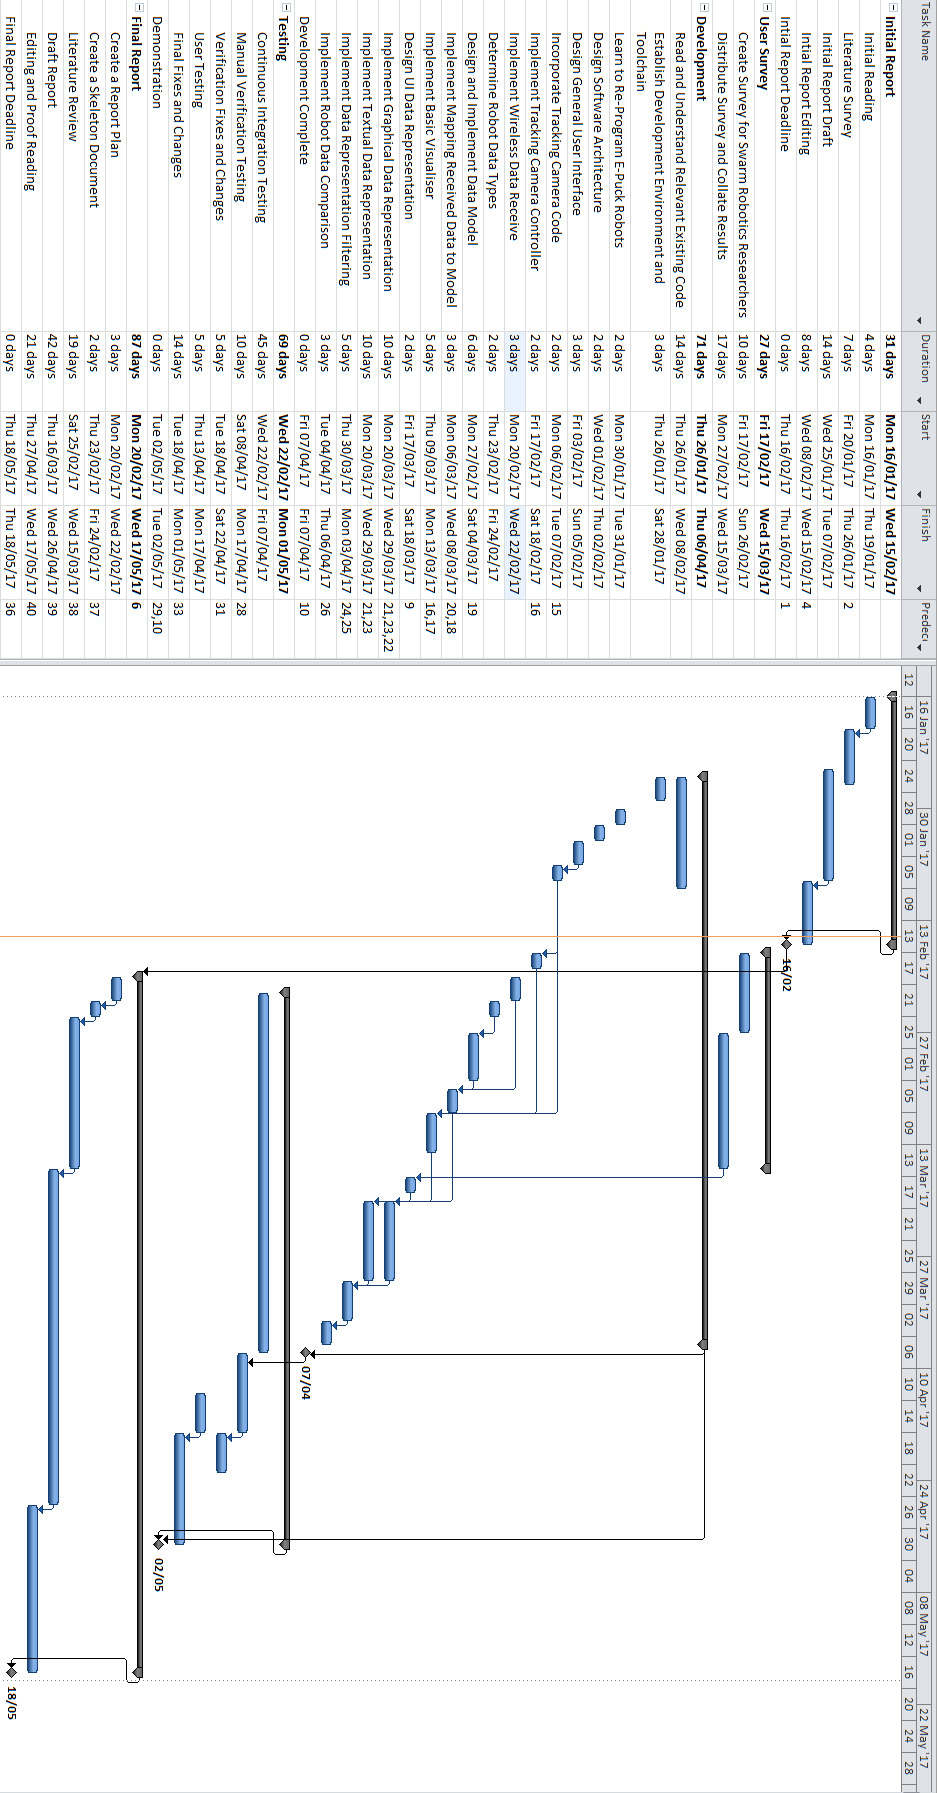
\includegraphics[scale=0.45]{Gant90.png}
	\caption{Gant Chart}
	\label{fig:GantChart}
	\end{center}
\end{figure}

\end{appendix}
\newpage

\begin{thebibliography}{1}
\bibitem{InspirationToApplication} E. Sahin, ``Swarm Robotics: From Sources of Inspiration to Domains of Application,'' in \textit{Swarm Robotics WS 2004}, E. S¸ahin and W.M. Spears, Eds. Springer, Berlin, LNCS 3342, 2005, pp. 10–20.

\bibitem{SwarmIntelligence} M. Dorigo and M. Birattari, ``Swarm intelligence,'' \textit{Scholarpedia}, vol. 2, no. 9, p. 1462, Sep. 2007. [Online]. Available: http://www.scholarpedia.org/article/Swarm\_intelligence. Accessed: Feb. 5, 2017.

\bibitem{EPuck} F. Mondada et al., ``The e-puck, a robot designed for education in engineering,'' in \textit{Proceedings of the 9th Conference on Autonomous Robot Systems and Competitions}, vol. 1, IPCB: Instituto Politécnico de Castelo Branco, 2009, pp. 59–65.

\bibitem{SelfOrganizing} M. Dorigo et al., ``Evolving self-organizing behaviors for a Swarm-Bot,'' \textit{Autonomous Robots}, vol. 17, no. 2/3, pp. 223–245, 2004.

\bibitem{PathFormation} S. Nouyan, ``Path formation and goal search in swarm robotics,'' DEA thesis, Faculty of Applied Sciences, Universite Libre de Bruxelles, Brussels, 2004.

\bibitem{FromSIToSR}G. Beni, ``From Swarm Intelligence to Swarm Robotics,'' in \textit{Swarm Robotics WS 2004}, E. S¸ahin and W.M. Spears, Eds. Springer, Berlin, LNCS 3342, 2005, pp. 1–9.

\bibitem{FromNaturaltoArtificial} E. Bonabeau, M. Dorigo, and G. Theraulaz, \textit{Swarm intelligence: From natural to artificial systems}. Oxford University Press, 1999.

\bibitem{HumanSwarmInteractionSurvey} A. Kolling, P. Walker, N. Chakraborty, K. Sycara and M. Lewis, ``Human Interaction With Robot Swarms: A Survey,'' in \textit{IEEE Transactions on Human-Machine Systems}, vol. 46, no. 1, 2016, pp. 9-26.

\bibitem{DesginingInterfaces} A. Rule and J. Forlizzi, ``Designing interfaces for multi-user, multi-robot systems,'' \textit{Proceedings of the seventh annual ACM/IEEE international conference on Human-Robot Interaction}, 2012, pp. 97–104.

\bibitem{InterfaceColour} R.E. Christ, ``Research for evaluating visual display codes: An emphasis on colour coding,'' in \textit{Information design: The design and evaluation of signs and printed materials}, R. Easterby and H. Zwaga, Eds. John Wiley and Sons, 1984, pp. 209-228.

\bibitem{InterfaceText} C. Carney, J. L. Campbell and E. A. Mitchell, \textit{In vehicle display icons and other information elements: Literature review}. U.S. Department of Transportation, Federal Highway Administration, USA; 1998.

\bibitem{AugmentedRealityDebuggingSystem} T. H. J. Collett and B. A. MacDonald, ``An augmented reality Debugging system for mobile robot software engineers,'' \textit{Journal of Software Engineering for Robotics}, vol. 1, no. 1, 2010, pp. 18–32.

\bibitem{Player} B. P. Gerkey, R. T. Vaughan, A. Howard, ``The Player/Stage Project: Tools for Multi-Robot and Distributed Sensor Systems,'' \textit{Proceedings of the 11th International Conference on Advanced Robotics}, 2003, pp. 317-323.

\bibitem{ARForPlayer} T. H. J. Collett and B. A. MacDonald, ``Augmented reality visualisation for player,'' \textit{Proceedings 2006 IEEE International Conference on Robotics and Automation}, 2006, pp. 3954-3959.

\bibitem{LEDSwarmAR} F. Ghiringhelli et al., ``Interactive Augmented Reality for understanding and analyzing multi-robot systems,'' \textit{2014 IEEE/RSJ International Conference on Intelligent Robots and Systems}, 2014, pp. 1195-1201.

\bibitem{AruCo} S. Garrido-Jurado et al., ``Automatic generation and Detection of Highly Reliable Fiducial Markers Under Occlusion'', \textit{Pattern Recognition}, vol. 47, no. 6, 2014, pp. 228 - 2292.

\bibitem{NASAApproach} NASA Software Engineering Laboratory, \textit{Recommended Approach to Software Development}. National Aeronautics and Space Administration, MD, USA; 1992. [Online]. Available: http://homepages.inf.ed.ac.uk/dts/pm/Papers/nasa-approach.pdf. Accessed: Feb. 5, 2017.

\bibitem{Agile} J. Highsmith and A. Cockburn, ``Agile software development: the business of innovation,'' in \textit{Computer}, vol. 34, no. 9, 2001, pp. 120-127.

\end{thebibliography}

\end{document}
